\documentclass[../zhang_thesis.tex]{subfiles}
\begin{document}

\chapter{Problem Setup}

%%%%%%%%%%%%%%%%%%%%%%%%%%%%%%%%%%%%%%%%%%%%%%%%%%%%%%%%%%%%%%%

\begin{figure}[b]
\centering
%\psfrag{i}[][]{$i_\text{cell}$}
\psfrag{v}[][]{$V_\text{cell}$}
\psfrag{+}[][]{$+$}
\psfrag{-}[][]{$-$}
\psfrag{R}[][]{$R_{sd}$}
\psfrag{Vs}[][]{$V_\text{SOC}$}
\psfrag{C}[][]{$C_\text{cap}$}
\psfrag{Vo}[][]{$V_\text{OC}$}
\psfrag{Vc}[][]{$V_\text{cell}$}
\psfrag{Rs}[][]{$R_s$}
\psfrag{Ra}[][]{$R_{ts}$}
\psfrag{Ca}[][]{$C_{ts}$}
\psfrag{Va}[][]{$V_{ts}$}
\psfrag{Rb}[][]{$R_{tl}$}
\psfrag{Cb}[][]{$C_{tl}$}
\psfrag{Vb}[][]{$V_{tl}$}

\centering
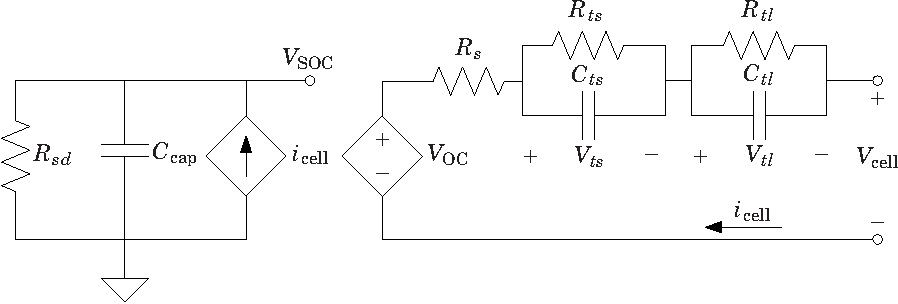
\includegraphics[width=\columnwidth]{batt_model}
\psfragfig[width=\columnwidth]{chapter-2/figures/batt_model}
\caption{Electrical-circuit battery model.}
\label{fig:batt_model}
\end{figure}

\section{Battery Model}
\label{sec:batt_mdl}

As discussed in the previous section, this thesis considers the electrical-circuit battery model proposed by Chen and Rinc\'on-Mora~\cite{chen06} and shown in \cref{fig:batt_model}. The left portion of the circuit models the capacity, SOC, and runtime, while the right portion models the transient i-v characteristics.  For convenience, the model is designed so that the SOC of the battery equals the voltage $V_\text{SOC}$, in volts. The parameters $C_\text{cap}$ and
$R_{sd}$ are assumed constant for a given battery and determine the capacity and self-discharge rate of the battery. The other parameters are all nonlinear functions of $V_\text{SOC}$ and determine the transient i-v response as well as the open-circuit voltage $V_\text{OC}$. From a typical TCL PL-383562 polymer lithium-ion battery, Chen and Rinc\'on-Mora extracted these parameters and fit them to curves, obtaining
\begin{gather}
    R_s(V_\text{SOC}) = 0.1562 e^{-24.37 V_\text{SOC}} + 0.07446 \label{eq:nl_param_1} \\
    R_{ts}(V_\text{SOC}) = 0.3208 e^{-29.14 V_\text{SOC}} + 0.04669 \\
    C_{ts}(V_\text{SOC}) = -752.9 e^{-13.51 V_\text{SOC}} + 703.6 \\
    R_{tl}(V_\text{SOC}) = 6.603 e^{-155.2 V_\text{SOC}} + 0.04984 \\
    C_{tl}(V_\text{SOC}) = -6056 e^{-27.12 V_\text{SOC}} + 4475 \\
    V_\text{OC}(V_\text{SOC}) = -1.031 e^{-35 V_\text{SOC}} + 3.685 + 0.2156 V_\text{SOC} - 0.1178 V_\text{SOC}^2 + 0.3201 V_\text{SOC}^3 \label{eq:nl_param_6}
\end{gather}
The resistance and capacitance parameters shown above are approximately constant for $\text{SOC}>0.2$ and change exponentially for $\text{SOC}<0.2$. The open-circuit voltage also changes exponentially for $\text{SOC}<0.2$ but is approximately linear for $\text{SOC}>0.2$. Note that the capacitances $C_{ts}$ and $C_{tl}$ are negative for SOC values close to zero, which is both unrealistic according to the experimental data collected by Chen and Rin\'on-Mora and problematic
mathematically. To solve this, a lower bound was placed on the $V_\text{SOC}$ input to the capacitance functions. Thus, for inputs below some threshold value $v_T$, the capacitances are adjusted to their value at that threshold, producing
\begin{align}
    \hat{C}_{ts}(V_\text{SOC}) &= \begin{cases}
        C_{ts}(V_\text{SOC}), & V_\text{SOC} \ge v_T \\
        C_{ts}(v_T), & V_\text{SOC} < v_T
        \end{cases} \label{eq:Cts_thres} \\
    \hat{C}_{tl}(V_\text{SOC}) &= \begin{cases}
        C_{tl}(V_\text{SOC}), & V_\text{SOC} \ge v_T \\
        C_{tl}(v_T), & V_\text{SOC} < v_T \label{eq:Ctl_thres}
        \end{cases}
\end{align}
The threshold $v_T$ was chosen based on the experimental data of Chen and Rin\'on-Mora, specifically so that the threshold capacitance values are approximately equal to the lowest such values measured by them. A threshold of $v_T=0.015$~V accomplishes this goal.

This study used the nonlinear parameters given by Chen and Rinc\'on-Mora for the implementation of a battery using their battery model in Matlab. In addition, the thresholding defined in \cref{eq:Cts_thres,eq:Ctl_thres} was used with $v_T=0.015$~V. The other, constant parameters were chosen to produce a capacity of 1~Ah and a self-discharge rate of 4\% per month. To do so, the capacitance $C_\text{cap}$ is calculated to hold the desired capacity
when $V_\text{SOC}=1$~V, and then the resistance $R_{sd}$ is set to produce the desired self-discharge rate. For a given capacity of $C^\dag$ in Ah, $C_\text{cap}$ needs to be
\begin{equation}
    C_\text{cap} = \frac{Q}{V_\text{SOC}} = \frac{C^\dag}{1~\text{V}} = 3600 C^\dag \,[\text{F}].
\end{equation}
Then, the resistance $R_{sd}$ is chosen so that the time constant $\tau=RC$ results in the desired drop of $\xi=0.04$ over $T=1$~month as follows
\begin{gather}
    V(t) = V_0 e^{-T/\tau} = V_0 (1-\xi) \\
    \tau = -T/\ln(1-\xi) = -2592000/\ln 0.96 \,[\text{s}].
\end{gather}
Then, $R_{sd}=\tau/C_\text{cap}$. Thus, the parameters are $C_\text{cap}=3600$~F and $R_{sd}=17.6376~\mathrm{k}\Omega$.

In order to simulate the use of the modeled battery, discharging and charging loads were implemented, as shown in \autorefs{fig:batt_loads}. For discharging, a resistive load $R_L$ is placed across the battery terminals, creating a discharge rate of $i_\text{cell}=V_\text{cell}/R_L$. For charging, a negative resistance $-R_L$, where $R_L>0$, is used, creating a charging current of $-i_\text{cell}=V_\text{cell}/R_L$. Thus, any arbitrary charging or discharging current can be set
by choosing the appropriate resistance $R_L$. Furthermore, an open circuit can be simulated by choosing $R_L$ sufficiently large so that $i_\text{cell}\approx 0$. Additional consideration has to be taken to ensure that the constant current and constant voltage charging conditions in standard charging procedure can be produced using a negative resistance. Typically, the specific battery modeled by the given parameters is charged at a rate of $C_5/5$ until a terminal voltage of $4.2$~V is reached, where $C_5/5$ is the discharge
rate at which a full battery is completely discharged in 5 hours~\cite{linden01_ch3}. Then, the battery is charged at a constant voltage of $4.2$~V until the charging current is below $C_5/20$. The constant current condition can be met by varying $R_L$ so that $V_\text{cell}/R_L$ stays constant, while the constant voltage condition is met by varying $R_L$ so that $i_\text{cell} R_L$ stays constant.

\begin{figure}[ht]
\centering
\begin{subfigure}[c]{0.4\textwidth}
    %\psfrag{i}[][]{$i_\text{cell}$}
\psfrag{v}[][]{$V_\text{cell}$}
\psfrag{+}[][]{$+$}
\psfrag{-}[][]{$-$}
\psfrag{R}[][]{$R_L$}

\centering
%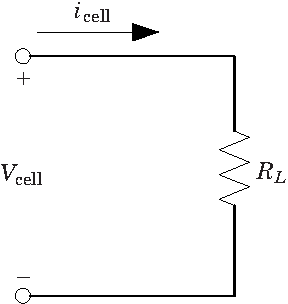
\includegraphics[width=0.75\columnwidth]{resistive_load}

    \centering
    \psfragfig[width=0.3\textwidth]{chapter-2/figures/resistive_load}
\end{subfigure}
\begin{subfigure}[c]{0.55\textwidth}
    %\psfrag{i}[][]{$i_\text{cell}$}
\psfrag{v}[][]{$V_\text{cell}$}
\psfrag{y}[][]{$V_o$}
\psfrag{+}[][]{$+$}
\psfrag{-}[][]{$-$}
\psfrag{R}[][]{$\lvert R_L \rvert$}
\psfrag{Ra}[][]{$R_1$}
\psfrag{Rb}[][]{$R_1$}

\centering
%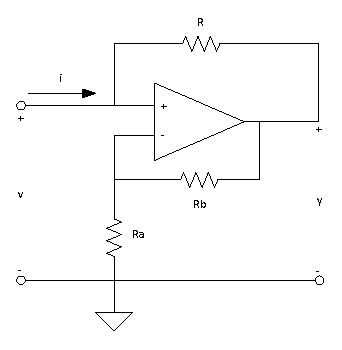
\includegraphics[width=0.9\columnwidth]{nrc}

    \centering
    \psfragfig[width=0.495\textwidth]{chapter-2/figures/nrc}
\end{subfigure}
\caption{Loads to (a) discharge and (b) charge the battery.}
\label{fig:batt_loads}
\end{figure}

This use of the load $R_L$ to control the current $i_\text{cell}$ means it is the input to the system. Moreover, the measurable outputs of the system are $V_\text{cell}$ and $i_\text{cell}$. However, since knowledge of one of them along with $R_L$ allows for the calculation of the other, the two outputs have a known relationship between them. Therefore, only one of the outputs is necessary to fully define the input-output relationship of the system. In this study, the voltage
$V_\text{cell}$ was chosen as the measured output as is typical for single-measurement battery system models.

For ease of numerical simulation, it is useful to find the state-space system for the circuit. The state-space representation is derived using the physical variable definition, in which the state variables are chosen to represent the voltages across the capacitors. Choosing $x_1=V_\text{SOC}$, $x_2=V_{ts}$, and $x_3=V_{tl}$ achieves this goal and results in the state-space representation
\begin{align}
    \dot{x}_1 &= - \frac{x_1}{R_{sd}C_\text{cap}} - \frac{V_\text{OC}(x_1)-x_2-x_3}{(R_s(x_1)+R_L)C_\text{cap}} + f_{w,1}(\mathbf{x},R_L,\mathbf{w}) \\
    \dot{x}_2 &= - \frac{x_2}{R_{ts}(x_1)C_{ts}(x_1)} + \frac{V_\text{OC}(x_1) - x_2 - x_3}{(R_s(x_1)+R_L)C_{ts}(x_1)} + f_{w,2}(\mathbf{x},R_L,\mathbf{w}) \\
    \dot{x}_3 &= - \frac{x_3}{R_{tl}(x_1)C_{tl}(x_1)} + \frac{V_\text{OC}(x_1) - x_2 - x_3}{(R_s(x_1)+R_L)C_{tl}(x_1)} + f_{w,3}(\mathbf{x},R_L,\mathbf{w}) \\
    V_\text{cell} &= \frac{V_\text{OC}(x_1) - x_2 - x_3}{1+R_s(x_1)/R_L} + f_v(\mathbf{x},R_L,\mathbf{v}),
\end{align}
where $R_L$ is the input to the system, $V_\text{cell}$ is the output, $f_w$ is the process noise function, $f_v$ is the measurement noise function, and the nonlinear parameters depending on $x_1$ are given by \crefrange{eq:nl_param_1}{eq:nl_param_6} along with the thresholding defined in \cref{eq:Cts_thres,eq:Ctl_thres}. It is obvious from this formulation that the system is nonlinear to both the input and the states. In order to establish the noise expressions, the types of
noise present in the battery have to first be determined.

This thesis assumes that the process and measurement noises in this system are due to thermal noise in the resistances for the internal impedance of the battery $R_s$, $R_{ts}$, and $R_{tl}$, and for the load $R_L$. This is motivated by measurements of the voltage noise in batteries conducted by Boggs et al.\ that showed the measured noise is mainly due to thermal noise since shot noise is suppressed by the correlation between the battery terminals~\cite{boggs95}. This thermal noise
is assumed to be Gaussian white noise with a power spectral density (PSD) of~\cite{stremler82}
\begin{equation}
    S_n(\omega) \cong 2kT\ \text{watts per Hz} \qquad \text{for} \qquad |\omega| \ll 2\pi kT/h,
\end{equation}
where $T$ is the temperature of the conducting medium in Kelvin, $k$ is the Boltzmann's constant, and $h$ is the Planck's constant. \cref{fig:batt_noisy} shows that the thermal noise due to the resistances is modeled as voltage sources in series with the resistances, with PSDs of $S_v(\omega)=2kTR$ for a corresponding resistance $R$. Using this definition, the noise functions are given by
\begin{figure}[b]
\centering
%\psfrag{i}[][]{$i_\text{cell}$}
\psfrag{v}[][]{$V_\text{cell}$}
\psfrag{+}[][]{$+$}
\psfrag{-}[][]{$-$}
\psfrag{Vo}[][]{$V_\text{OC}$}
\psfrag{Vc}[][]{$V_\text{cell}$}
\psfrag{Rs}[][]{$R_s$}
\psfrag{Ra}[][]{$R_{ts}$}
\psfrag{Ca}[][]{$C_{ts}$}
\psfrag{Va}[][]{$V_{ts}$}
\psfrag{Rb}[][]{$R_{tl}$}
\psfrag{Cb}[][]{$C_{tl}$}
\psfrag{Vb}[][]{$V_{tl}$}
\psfrag{RL}[][]{$R_L$}
\psfrag{vns}[][]{$v_{n_s}$}
\psfrag{vts}[][]{$v_{n_{ts}}$}
\psfrag{vtl}[][]{$v_{n_{tl}}$}
\psfrag{vnl}[][]{$v_{n_L}$}

\centering
%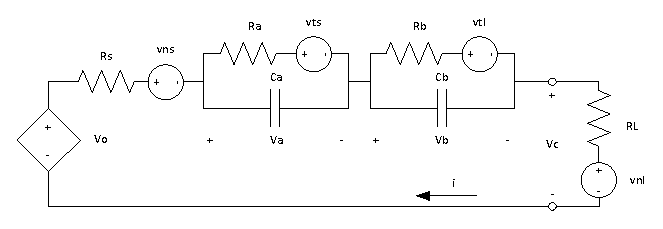
\includegraphics[width=\columnwidth]{batt_noisy}

\psfragfig[width=\columnwidth]{chapter-2/figures/batt_noisy}
\caption{Modeling of thermal noise in resistances as voltage sources in series with the resistances.}
\label{fig:batt_noisy}
\end{figure}
\begin{align}
    f_{w,1} &= \frac{v_{n_s}+v_{n_L}}{(R_s(x_1)+R_L)C_\text{cap}} \\
    f_{w,2} &= \frac{v_{n_{ts}}}{R_{ts}(x_1)C_{ts}(x_1)} - \frac{v_{n_s}+v_{n_L}}{(R_s(x_1)+R_L)C_{ts}(x_1)} \\
    f_{w,3} &= \frac{v_{n_{tl}}}{R_{tl}(x_1)C_{tl}(x_1)} - \frac{v_{n_s}+v_{n_L}}{(R_s(x_1)+R_L)C_{tl}(x_1)} \\
    f_v &= - \frac{v_{n_s}+v_{n_L}}{1+R_s(x_1)/R_L}.
\end{align}
It can be seen that the resistances change over time, which causes the PSD of the sources $v_n$ to also change. For the purposes of modeling, it is useful to define noise variables that have constant PSDs. Using the square root of the power supplied by the noise sources as the noise variables accomplishes this goal and produces the variables $w_1=v_{n_s}/\sqrt{R_s}$, $w_2=v_{n_{ts}}/\sqrt{R_{ts}}$, $w_3=v_{n_{tl}}/\sqrt{R_{tl}}$, and $w_4=v_{n_L}/\sqrt{|R_L|}$ along with
$v_1=v_{n_s}/\sqrt{R_s}$ and $v_2=v_{n_L}/\sqrt{|R_L|}$, which all have
constant PSDs of $2kT$. Note the use of the absolute value of $R_L$ in the definition of $w_4$ and $v_2$, since $R_L$ can become negative. In the case of $R_L<0$, their PSDs remain at $2kT$ while the sign of $v_{n_L}$ is negated, which is implemented in the system using the signum function, defined as
\begin{equation}
    \sgn(x) := \begin{cases}
        -1 & \text{if } x<0 \\
        0 & \text{if } x=0 \\
        1 & \text{if } x>0.
    \end{cases}
\end{equation}
Then, the state space representation of the system becomes
\begin{align}
    \dot{x}_1 &= - \frac{x_1}{R_{sd}C_\text{cap}} - \frac{V_\text{OC}(x_1) - x_2 - x_3 - \sqrt{R_s(x_1)}w_1 - \sgn(R_L)\sqrt{|R_L|}w_4}{(R_s(x_1)+R_L)C_\text{cap}} \\
    \dot{x}_2 &= - \frac{x_2 - \sqrt{R_{ts}(x_1)}w_2}{R_{ts}(x_1)C_{ts}(x_1)} + \frac{V_\text{OC}(x_1) - x_2 - x_3 - \sqrt{R_s(x_1)}w_1 - \sgn(R_L)\sqrt{R_L}w_4}{(R_s(x_1)+R_L)C_{ts}(x_1)} \\
    \dot{x}_3 &= - \frac{x_3 - \sqrt{R_{tl}(x_1)}w_3}{R_{tl}(x_1)C_{tl}(x_1)} + \frac{V_\text{OC}(x_1) - x_2 - x_3 - \sqrt{R_s(x_1)}w_1 - \sgn(R_L)\sqrt{R_L}w_4}{(R_s(x_1)+R_L)C_{tl}(x_1)} \\
    V_\text{cell} &= \frac{V_\text{OC}(x_1) - x_2 - x_3 - \sqrt{R_s(x_1)}v_1 - \sgn(R_L)\sqrt{R_L}v_2}{1+R_s(x_1)/R_L}.
\end{align}
It can be seen that the system can be written in the form
\begin{align}
    \dot{\vx}(t) &= \vf(\vx(t),\vu(t),\vw(t)) \\
    \vz(t) &= \vh(\vx(t),\vu(t),\vv(t)),
\end{align}
where $\vx$ is the state, $\vu$ is the input, $\vf$ is the nonlinear differential equation for the state, $\vh$ is the nonlinear measurement function, and $\vw$ and $\vv$ are Wiener processes used to represent the integral of the Gaussian white-noise noise sources. It is useful to find the derivatives of $\vf$ and $\vh$ with respect to $\vx$, $\vw$, and $\vv$ for use with the filters. This thesis defines the Jacobians $F=\partial\vf/\partial\vx$, $H=\partial\vh/\partial\vx$,
$L=\partial\vf/\partial\vw$, and $M=\partial\vh/\partial\mathbf{v}$. Their equations are
\begin{align}
    F & = \scalemath{0.9}{ \left[ \begin{multlined} \begin{array}{@{}c}
        \dfrac{-1}{R_{sd}C_\text{cap}} + \dfrac{\splitfrac{(Voc-x_2-x_3)R_s'}{- (R_s+R_L)V_\text{OC}'}}{(R_s+R_L)^2 C_\text{cap}} \\[3ex]
        \dfrac{(R_{ts}C_{ts})' x_2}{R_{ts}C_{ts}} + \dfrac{\splitfrac{(R_s+R_L)C_{ts}V_\text{OC}'}{- (Voc-x_2-x_3)\big[(R_s+R_L)C_{ts}\big]'}}{\big[(R_s+R_L)C_{ts}\big]^2}  \\[3ex]
        \dfrac{(R_{tl}C_{tl})' x_3}{R_{tl}C_{tl}} + \dfrac{\splitfrac{(R_s+R_L)C_{tl}V_\text{OC}'}{- (Voc-x_2-x_3)\big[(R_s+R_L)C_{tl}\big]'}}{\big[(R_s+R_L)C_{tl}\big]^2} 
        \end{array} \\
        \begin{array}{@{\hspace{1in}\ldots\hspace{1in}}cc@{}}
            \dfrac{1}{(R_s+R_L)C_\text{cap}} & \dfrac{1}{(R_s+R_L)C_\text{cap}} \\[3ex]
            \dfrac{-1}{R_{ts}C_{ts}}+\dfrac{-1}{(R_s+R_L)C_{ts}} & \dfrac{-1}{(R_s+R_L)C_{ts}} \\[3ex]
            \dfrac{-1}{(R_s+R_L)C_{tl}} & \dfrac{-1}{R_{tl}C_{tl}}+\dfrac{-1}{(R_s+R_L)C_{tl}}
        \end{array} \end{multlined} \right] } \\
    H & = \begin{bmatrix}
            \dfrac{\splitfrac{(1+R_s/R_L)V_\text{OC}'}{- (V_\text{OC}-x_2-x_3)R_s'/R_L}}{(1+R_s/R_L)^2} & \dfrac{-1}{1+R_s/R_L} & \dfrac{-1}{1+R_s/R_L}
        \end{bmatrix} \\[3ex]
    L & = \begin{bmatrix}
            \dfrac{\sqrt{R_s}}{(R_s+R_L)C_\text{cap}} & 0 & 0 & \dfrac{\sgn{R_L}\sqrt{|R_L|}}{(R_s+R_L)C_\text{cap}} \\[3ex]
            \dfrac{-\sqrt{R_s}}{(R_s+R_L)C_\text{cap}} & \dfrac{\sqrt{R_{ts}}}{R_{ts}C_{ts}} & 0 & \dfrac{-\sgn{R_L}\sqrt{|R_L|}}{(R_s+R_L)C_\text{cap}} \\[3ex]
            \dfrac{-\sqrt{R_s}}{(R_s+R_L)C_\text{cap}} & 0 & \dfrac{\sqrt{R_{tl}}}{R_{tl}C_{tl}} & \dfrac{-\sgn{R_L}\sqrt{|R_L|}}{(R_s+R_L)C_\text{cap}}
        \end{bmatrix} \\[3ex]
    M & = \begin{bmatrix}
            %\dfrac{-\sqrt{R_s}}{(R_s+R_L)C_\text{cap}} & \dfrac{-\sgn{R_L}\sqrt{|R_L|}}{(R_s+R_L)C_\text{cap}}
            \dfrac{-\sqrt{R_s}}{1+R_s/R_L} & \dfrac{-\sgn{R_L}\sqrt{|R_L|}}{1+R_s/R_L}
        \end{bmatrix} ,
\end{align}
where $(\ )'$ indicates derivation with respect to $x_1$ and the dependence on $x_1$ has been omitted due to space constraints. Furthermore, it is useful to find the Hessian of $\vf$ with respect to $\vx$. Due to symmetry and $\partial^2 f_k/\partial x_i\partial x_j = 0$ for $i,j=2,3$, only the first column of each tensor component of the Hessian is given. The resultant Hessian is
\begin{align}
    \frac{\partial^2 f_1}{\partial x_i \partial x_1} & = \begin{bmatrix}
            \dfrac{\splitfrac{(R_s+R_L)\big[(V_\text{OC}-x_2-x_3)R_s''-(R_s+R_L)V_\text{OC}''\big]}{- 2R_s' \big[(V_\text{OC}-x_2-x_3)R_s' - (R_s+R_L)V_\text{OC}'\big]}}{(R_s+R_L)^3 C_\text{cap}} \\[3ex]
            \dfrac{-R_s'}{(R_s+R_L)^2 C_\text{cap}} \\[3ex]
            \dfrac{-R_s'}{(R_s+R_L)^2 C_\text{cap}}
        \end{bmatrix} \\
    \frac{\partial^2 f_2}{\partial x_i \partial x_1} & = \scalemath{0.8}{ \begin{bmatrix}
            \dfrac{\splitfrac{\big\{R_{ts}C_{ts}(R_{ts}C_{ts})''}{- \big[(R_{ts}C_{ts})'\big]^2\big\}x_2}}{(R_{ts}C_{ts})^2} + \dfrac{\splitfrac{(R_s+R_L)C_{ts}\big\{(R_s+R_L)C_{ts}V_\text{OC}'' - (V_\text{OC}-x_2-x_3)\big[(R_s+R_L)C_{ts}\big]''\big\}}{+ 2 \big[(R_s+R_L)C_{ts}\big]' \big\{(R_s+R_L)C_{ts}V_\text{OC}' - (Voc-x_2-x_3)\big[(R_s+R_L)C_{ts}\big]'\big\}}}{\big[(R_s+R_L)C_{ts}\big]^3} \\[3ex]
            \dfrac{(R_{ts}C_{ts})'}{R_{ts}C_{ts}}+\dfrac{\big[(R_s+R_L)C_{ts}\big]'}{\big[(R_s+R_L)C_{ts}\big]^2} \\[3ex]
            \dfrac{\big[(R_s+R_L)C_{ts}\big]'}{\big[(R_s+R_L)C_{ts}\big]^2}
        \end{bmatrix} } \\
    \frac{\partial^2 f_3}{\partial x_i \partial x_1} & = \scalemath{0.8}{ \begin{bmatrix}
            \dfrac{\splitfrac{\big\{R_{tl}C_{tl}(R_{tl}C_{tl})''}{- \big[(R_{tl}C_{tl})'\big]^2\big\}x_3}}{(R_{tl}C_{tl})^2} + \dfrac{\splitfrac{(R_s+R_L)C_{tl}\big\{(R_s+R_L)C_{tl}V_\text{OC}'' - (V_\text{OC}-x_2-x_3)\big[(R_s+R_L)C_{tl}\big]''\big\}}{+ 2 \big[(R_s+R_L)C_{tl}\big]' \big\{(R_s+R_L)C_{tl}V_\text{OC}' - (Voc-x_2-x_3)\big[(R_s+R_L)C_{tl}\big]'\big\}}}{\big[(R_s+R_L)C_{tl}\big]^3} \\[3ex]
            \dfrac{\big[(R_s+R_L)C_{tl}\big]'}{\big[(R_s+R_L)C_{tl}\big]^2} \\[3ex]
            \dfrac{(R_{tl}C_{tl})'}{R_{tl}C_{tl}}+\dfrac{\big[(R_s+R_L)C_{tl}\big]'}{\big[(R_s+R_L)C_{tl}\big]^2}
        \end{bmatrix} }
\end{align}
Furthermore, based on the forms of the Jacobians $L$ and $M$, the battery system can be written as
\begin{align}
    \dot{\vx}(t) &= \vf(\vx(t),\vu(t)) + L(\vx(t),\vu(t)) \sqrt{Q} \vw(t) \label{eq:ct_diff} \\
    \vz_k &= \vh(\vx_k,\vu_k) + M(\vx_k,\vu_k) \sqrt{R} \vv(t_k) \delta,
\end{align}
where the diagonals of $Q=2kT I_4$ and $R=2kT I_2$ are the values of the PSDs of the noise sources, $I_n$ is the $n\times n$ identity matrix, and $\delta=t_k-t_{k-1}$ is the time step for the discrete-time measurements. Note that the state dynamics are in continuous-time. The discretization of the continuous-time dynamics for use with the filters is discussed in the next section. Additionally, for convenience, the quantity $\sqrt{R} \vv(t_k) \delta$ will be referred to as $\vv_k$. Note
that $\vv_k\sim\mathcal{N}(0,\delta R)$ is a Gaussian random variable whose covariance is the PSD of the measurement noise sources scaled by the time step.

\section{Discretization of System Dynamics}
\label{sec:discret}

In the prediction phases of the filters, the expected value of the continuous-time differential equation for the state in \cref{eq:ct_diff} needs to be computed. In order to find the state $\vx(t_k)$ from the state $\vx(t_{k-1})$, assuming the input is constant, the equation can be solved numerically. Assume that the discretized system has the form
\begin{equation}
    \dot{\vx}_k = \vf_d(\vx_{k-1},\vu_k) + L(\vx_{k-1},\vu_k) \sqrt{Q} \vw(t_k) \delta.
\end{equation}
For convenience, let $\vw_k=\sqrt{Q} \vw(t_k) \delta$, where $\delta=t_k-t_{k-1}$ is the time step. Note that $\vw_k\sim\mathcal{N}(0,\delta Q)$ is a Gaussian random variable whose covariance is the PSD of the process noise sources scaled by the time step. Additionally, recall that $\vv_k$ is also a Gaussian random variable. Then, the discrete-time system is given by
\begin{align}
    \dot{\vx}_k &= \vf_d(\vx_{k-1},\vu_k) + L(\vx_{k-1},\vu_k) \vw_k \label{eq:dt1} \\
    \vz_k &= \vh(\vx_k,\vu_k) + M(\vx_k,\vu_k) \vv_k, \label{eq:dt2}
\end{align}
where $\vw_k\sim\mathcal{N}(0,2kT\delta I_4)$ and $\vv_k\sim\mathcal{N}(0,2kT\delta I_2)$. The scaling of the covariances by $\delta$ is from the conversion of the continuous-time Wiener processes to the discrete-time Gaussian random variables.

S\"arkk\"a and Solin state that a linearized discretization approach, in which the continuous-time system is first discretized and then approximated as Gaussian, tends to work better than a
discretized linearization approach, in which the system is first approximated as a Gaussian process and then discretized~\cite{sarkka12}. This thesis follows this guideline and performs the prediction using linearized approximations of a discretization of the continuous-time dynamics. To increase the accuracy of the discretized integration in the prediction phase, the sampling period is divided into $M$ steps of equal length and the integration is performed in $M$ steps. The motivation
for this iterated integration comes from the definition of order for an It\^o-Taylor expansion of a stochastic differential equation. An expansion is said to be strongly convergent with order $\beta$ if for any positive integer $M$ and time interval $[t_{k-1},t_k]$, the error of the $M$-step approximation satisfies~\cite{kloeden99}
\begin{equation}
    E \left[ \sup_{t\in[t_{k-1},t_k]} |\vx(t) - \hat{\vx}^{(M)}(t) \right] \le \lambda (\delta^{(M)})^\beta,
\end{equation}
where $\vx(t)$ is exact solution, $\vx^{(M)}(t)$ is the $M$-step approximation, $\delta=(t_k-t_{k-1})/M$ and $\lambda$ is a constant uniform in $M$. It can be seen that the error of the approximation decreases as the number of integration steps $M$ increases.

Furthermore, note that the system is extremely stiff based the definition of the stiffness ratio as the ratio of the largest eigenvalue of $F$ to its smallest eigenvalue, where $F$ is the Jacobian of the dynamics $\vf(\mathbf{x},\mathbf{u})$; when the stiffness ratio is much greater than unity, the system is stiff~\cite{lambert91,brugnano11}. From EIS studies of batteries, the major chemical processes have widely differing time constants; low frequency mass transport effects like
diffusion are on the order of $10^{-6}$ to $10^0$ Hz, middle frequency effects caused by charge transfer and the electrochemical double layer are on the order of $10^0$ to $10^3$ Hz, and the high frequency conductance and skin effects are on the order of $10^3$ to $10^4$ Hz~\cite{jossen06}. Therefore, the approximate stiffness ratio is $10^{10} \gg 1$, and the system is stiff. As a result of the stiffness, any numerical integration method needs to be A-stable, i.e.\ the method
converges for all systems whose eigenvalues have negative real parts. For example, simulation results show that the fourth-order Runge-Kutta method diverges even at step sizes $<10^{-2}$ seconds.

This thesis uses the linearized discretization approach proposed by Mazzoni, in which the differential equation is first discretized and then approximated using Taylor series expansion~\cite{mazzoni07}. This approach has the advantage of A-stability. The discretization is performed using the trapezoidal approximation (Heun's method) of \cref{eq:ct_diff}, where $E[\vw_k]=0$ is used so that only the integration of $\vf$ needs to be considered. For convenience, denote the value of a
quantity at time $t_k$ using the subscript $k$ and assume that $\delta=t_k-t_{k-1}$ is the time step. Then, the approximation produces
\begin{equation}
    \vx_k \approx \vx_{k-1} + \frac{1}{2} \big( \vf(\vx_{k-1},\vu_k) + \vf(\vx_k,\vu_k) \big) \delta.
\end{equation}
The vector field $\vf$ at $\vx_k$ is approximated by first-order Taylor expansion around $\vx_{k-1}$, giving
\begin{equation}
    \vx_k \approx \vx_{k-1} + \vf(\vx_{k-1},\vu_k)\delta + \frac{1}{2} F(\vx_{k-1},\vu_k) \left( \vx_k - \vx_{k-1} \right) \delta,
\end{equation}
where $F(\vx_{k-1},\vu_k)$ is the Jacobian of $\vf$ at $\vx_{k-1}$. Solving for $\vx_k$ yields
\begin{equation}
    \vx_k \approx \vx_{k-1} + \left( I - F(\vx_{k-1},\vu_k) \frac{\delta}{2} \right)^{-1} \vf(\vx_{k-1},\vu_k) \delta,
\end{equation}
with the identity matrix $I$. This Taylor-Heun scheme uses linear Taylor expansion of $f$ rather than then Euler prediction of the standard Heun scheme. It is convergent with order $\mathcal{O}(\delta^2)$ and A-stable~\cite{mazzoni07}. Furthermore, this approximation is equivalent to the It\^o-Taylor expansion of order $\beta=0.5$~\cite{kloeden99}. This means the accuracy of the integration can be improved by iterating the integration over multiple steps, using a procedure similar to that of
S\"arkk\"a~\cite{sarkka12}, as follows. Choose some positive integer $M$ and let $\vx^{(i)}_{k-1}$ denote the $i$th iteration of the $M$-step integration method from $\vx_{k-1}$ to $\vx_k$, where $i=1,\dots,M$. Note that $\vx^{(0)}_{k-1}=\vx_{k-1}$ and $\vx^{(M)}_{k-1}=\vx_k$. Additionally, let $\delta=(t_k-t_{k-1})/M$. Then, the following procedure is iterated from $i=1$ to $M$:
\begin{equation}
    \vx^{(i)}_{k-1} = \vx^{(i-1)}_{k-1} + \left( I - F(\vx^{(i-1)}_{k-1},\vu_k) \frac{\delta}{2} \right)^{-1} \vf(\vx^{(i-1)}_{k-1},\vu_k) \delta.
\end{equation}
This thesis refers to each step of the $M$-step integration procedure as
\begin{equation}
    \vx_{k-1}^{(i)} = \vf_d(\vx_{k-1}^{(i-1)},\vu_k,\delta,i),
    \label{eq:mstep_int}
\end{equation}
where $\delta==(t_k-t_{k-1})/M$ is the time step for each iteration and $i=1,\dots,M$ is the current iteration. For convenience, the result of the iterative integration is referred to as $\vx_k=\vf_d(\vx_{k-1},\vu_k)$. This iterated numerical integration was used in the prediction steps of the filters.

\section{Simulation Setup}

In order to simulate the stochastic system, the covariances of the noises as well as their generation and simulation methods have to be determined. This thesis assumed that a standard temperature of $T=290$~Kelvin. Therefore, the PSDs of the white Gaussian noise processes are $\sigma^2=2kT=8.0078\times 10^{-21}$~W/Hz. The covariances of the Gaussian noises in the discrete-time system are scaled versions of the PSDs. Specifically, the value of the constant PSDs are scaled by the
discrete time step $\delta$. Note that due to the use of a multi-step integration method for the discretization of the dynamics, the time step is scaled by the number of integration steps $M$. Therefore, the covariances in \cref{eq:dt1,eq:dt2} are
\begin{align}
    Q &= 2kT\delta I_4 / M \\
    R &= 2kT\delta I_2.
\end{align}
Furthermore, to better differentiate the performance of the filters, additional measurement noise was introduced assuming an oscilloscope was used to perform the measurement.
Specifically, consider the Tektronix TBS1022 oscilloscope with a DC gain accuracy of $\pm 3\%$ of the full range. Based on numerical simulations, an approximate range of 4~V peak-to-peak is necessary to fully capture the range of possible $V_\text{cell}$ values, resulting in a measurement inaccuracy of $\pm 0.12$~V. This noise is assumed to be normally distributed with the range laying within three standard deviations. Thus, an additional measurement noise variable $v_3$ is introduced with
a variance of
\begin{equation}
    \sigma_{v_3}^2 = \left( \frac{0.12~\text{V}}{3} \right)^2 = 0.0016~\text{V}^2.
\end{equation}
Note that this value already takes into account the discrete-time measurement. Then, the new measurement covariance matrix is
\begin{equation}
    R = \mathrm{diag}(2kT\delta,2kT\delta,0.0016),
\end{equation}
and the corresponding Jacobian $M=(\partial h/\partial\mathbf{v})$ is
\begin{equation}
    M = \begin{bmatrix}
         \dfrac{-\sqrt{R_s}}{(R_s+R_L)C_\text{cap}} & \dfrac{-\sgn{R_L}\sqrt{|R_L|}}{(R_s+R_L)C_\text{cap}} & 1
        \end{bmatrix} .
\end{equation}
In order to numerically simulate the effect of white noise on a system, the simulation time step must be sufficiently smaller than the time constant of the fastest battery process. This is approximated as the product of the constant terms of the functions for $R_{ts}$ and $C_{ts}$, halved to satisfy Nyquist conditions. Then, the simulation time step is taken to be $1/100$ of the calculated maximum time step, as suggested by Matlab documentation~\cite{matlab}. Thus, the simulations used a time step of
\begin{equation}
    \delta_\text{sim} = \frac{R_{ts,\text{const.}}C_{ts,\text{const.}}}{200} = \frac{0.04669\times 703.6}{200} = 0.164255~\text{s}.
\end{equation}
Simulation showed that the resulting time step is sufficiently small to capture the effects of the white noise, i.e.\ further reducing the step size had negligible effect. With the chosen step size, the noise is simulated as band-limited white Gaussian noise with a correlation time equal to the step size. At each time step, the noise values for the process noise sources are generated using random number generators producing normally-distributed numbers with means of zero and variances
equal to the diagonals of the covariance matrix divided by the correlation time. The scaling of the variance by the correlation time ensures the response of the system to the approximate white noise has the same covariance as it would have to actual white noise. Note that the measurement noise is bandlimited not by the system but by the measurement device, in this case an oscilloscope. Thus, the calculated variance already takes into account the measurement bandwidth of the oscilloscope and
scaling is unnecessary.

The simulation of the battery was done in a 64-bit installation of MATLAB 2012b on a computer running 64-bit Windows 7. For reproducibility, the random number generators were seeded with predictable numbers. This was done in MATLAB by first seeding the main random number generator with a seed of 0. Then, for each Monte Carlo trial, five positive integers were generated, for the five noise sources, with the integers uniformly distributed between 1 and $2^{32}-1$. These integers were used to seed the random number generators in a Simulink model. The use of the Simulink model allows for the
random number generators to be easily seeds with different integers and does not affect the predictable sequence in MATLAB.

\begin{figure}[htb]
\centering
%% generated by laprint.m
%
%
% text strings:
\psfrag{s01}[t][t]{\color[rgb]{0,0,0}\setlength{\tabcolsep}{0pt}\begin{tabular}{c}Time [hours]\end{tabular}}%
\psfrag{s02}[b][b]{\color[rgb]{0,0,0}\setlength{\tabcolsep}{0pt}\begin{tabular}{c}$R_L\ [\Omega]$\end{tabular}}%
%
% xticklabels:
\psfrag{x01}[t][t]{0}%
\psfrag{x02}[t][t]{0.1}%
\psfrag{x03}[t][t]{0.2}%
\psfrag{x04}[t][t]{0.3}%
\psfrag{x05}[t][t]{0.4}%
\psfrag{x06}[t][t]{0.5}%
\psfrag{x07}[t][t]{0.6}%
\psfrag{x08}[t][t]{0.7}%
\psfrag{x09}[t][t]{0.8}%
\psfrag{x10}[t][t]{0.9}%
\psfrag{x11}[t][t]{1}%
\psfrag{x12}[t][t]{0}%
\psfrag{x13}[t][t]{5}%
\psfrag{x14}[t][t]{10}%
\psfrag{x15}[t][t]{15}%
\psfrag{x16}[t][t]{20}%
\psfrag{x17}[t][t]{25}%
\psfrag{x18}[t][t]{30}%
%
% yticklabels:
\psfrag{v01}[r][r]{0}%
\psfrag{v02}[r][r]{0.1}%
\psfrag{v03}[r][r]{0.2}%
\psfrag{v04}[r][r]{0.3}%
\psfrag{v05}[r][r]{0.4}%
\psfrag{v06}[r][r]{0.5}%
\psfrag{v07}[r][r]{0.6}%
\psfrag{v08}[r][r]{0.7}%
\psfrag{v09}[r][r]{0.8}%
\psfrag{v10}[r][r]{0.9}%
\psfrag{v11}[r][r]{1}%
\psfrag{v12}[r][r]{-25}%
\psfrag{v13}[r][r]{-20}%
\psfrag{v14}[r][r]{-15}%
\psfrag{v15}[r][r]{-10}%
\psfrag{v16}[r][r]{-5}%
\psfrag{v17}[r][r]{0}%
\psfrag{v18}[r][r]{5}%
\psfrag{v19}[r][r]{10}%
\psfrag{v20}[r][r]{15}%
\psfrag{v21}[r][r]{20}%
\psfrag{v22}[r][r]{25}%
%
% Figure:
%
% End input.tex

%\psfragfig{chapter-2/figures/input2}
\pstool[width=15cm]{chapter-2/figures/input}{% generated by laprint.m
%
%
% text strings:
\psfrag{s01}[t][t]{\color[rgb]{0,0,0}\setlength{\tabcolsep}{0pt}\begin{tabular}{c}Time [hours]\end{tabular}}%
\psfrag{s02}[b][b]{\color[rgb]{0,0,0}\setlength{\tabcolsep}{0pt}\begin{tabular}{c}$R_L\ [\Omega]$\end{tabular}}%
%
% xticklabels:
\psfrag{x01}[t][t]{0}%
\psfrag{x02}[t][t]{0.1}%
\psfrag{x03}[t][t]{0.2}%
\psfrag{x04}[t][t]{0.3}%
\psfrag{x05}[t][t]{0.4}%
\psfrag{x06}[t][t]{0.5}%
\psfrag{x07}[t][t]{0.6}%
\psfrag{x08}[t][t]{0.7}%
\psfrag{x09}[t][t]{0.8}%
\psfrag{x10}[t][t]{0.9}%
\psfrag{x11}[t][t]{1}%
\psfrag{x12}[t][t]{0}%
\psfrag{x13}[t][t]{5}%
\psfrag{x14}[t][t]{10}%
\psfrag{x15}[t][t]{15}%
\psfrag{x16}[t][t]{20}%
\psfrag{x17}[t][t]{25}%
\psfrag{x18}[t][t]{30}%
%
% yticklabels:
\psfrag{v01}[r][r]{0}%
\psfrag{v02}[r][r]{0.1}%
\psfrag{v03}[r][r]{0.2}%
\psfrag{v04}[r][r]{0.3}%
\psfrag{v05}[r][r]{0.4}%
\psfrag{v06}[r][r]{0.5}%
\psfrag{v07}[r][r]{0.6}%
\psfrag{v08}[r][r]{0.7}%
\psfrag{v09}[r][r]{0.8}%
\psfrag{v10}[r][r]{0.9}%
\psfrag{v11}[r][r]{1}%
\psfrag{v12}[r][r]{-25}%
\psfrag{v13}[r][r]{-20}%
\psfrag{v14}[r][r]{-15}%
\psfrag{v15}[r][r]{-10}%
\psfrag{v16}[r][r]{-5}%
\psfrag{v17}[r][r]{0}%
\psfrag{v18}[r][r]{5}%
\psfrag{v19}[r][r]{10}%
\psfrag{v20}[r][r]{15}%
\psfrag{v21}[r][r]{20}%
\psfrag{v22}[r][r]{25}%
%
% Figure:
%
% End input.tex
}
\caption{Input load $R_L$ on the battery.}
\label{fig:input}
\end{figure}

Then, the battery was simulated using a Simulink model with the fourth-order Runge-Kutta method and an initial condition of $x_0=[1,0,0]^\top$. A total of 100 Monte Carlo runs of the battery were performed with seed values for the noise sources generated using the method mentioned in the previously. \cref{fig:input} shows the input load on the battery system, where the values off the graph are idle periods, simulated using a very large input of $R_L=10^{10}~\Omega$ so that the battery
current is approximately zero. It can be seen that the input is piecewise constant. This input was chosen to to test the performance of the filters by gradually increasing the strength of the nonlinear rate-capacity and recovery effects. Note that care was taken to ensure the SOC remained within the range of zero to one, so discharge and charge times could not always be equal. Initially, the battery is idle for 10 minutes to allow the estimated covariances of the filters to converge. Then, the
battery is discharged and charged at $R_L=20~\Omega$ for 290 and 270 minutes, respectively. The resulting low current from this load is approximately the testing current $C_5/5$ used to determine battery capacity, as discussed in \cref{sec:batt_mdl}. In order to increase the strength of the nonlinear effects, the absolute value of the current was increased by decreasing the input to $R_L=10~\Omega$ and discharging and charging for 150 minutes, each. Then, the input was further reduced to
$R_L=5~\Omega$ and discharged and charged for 80 minutes and 70 minutes, respectively. Next, the battery was discharged and charged at $R_L=4~\Omega$ for 60 minutes, each. Following were discharge and charge periods at $R_L=2~\Omega$ for 35, 25, 25, 20, 25, 25, 20, and 15 minutes. The high current results in very strong rate-capacity effects. Finally, the battery was rested for 70 minutes, discharged at $R_L=2~\Omega$ for 25 minutes, rested for 75 minutes, and charged at $R_L=10~\Omega$
for 135 minutes. The two resting periods should show the strongest recovery effect. The total input time is 1635 minutes. The SOC and the noisy measurement of $V_\text{cell}$ resulting from the given input is shown one Monte Carlo trial in \cref{fig:soc,fig:meas}, respectively.

\begin{figure}[htb]
\centering
%% This file is generated by the MATLAB m-file laprint.m. It can be included
% into LaTeX documents using the packages graphicx, color and psfrag.
% It is accompanied by a postscript file. A sample LaTeX file is:
%    \documentclass{article}\usepackage{graphicx,color,psfrag}
%    \begin{document}% This file is generated by the MATLAB m-file laprint.m. It can be included
% into LaTeX documents using the packages graphicx, color and psfrag.
% It is accompanied by a postscript file. A sample LaTeX file is:
%    \documentclass{article}\usepackage{graphicx,color,psfrag}
%    \begin{document}% This file is generated by the MATLAB m-file laprint.m. It can be included
% into LaTeX documents using the packages graphicx, color and psfrag.
% It is accompanied by a postscript file. A sample LaTeX file is:
%    \documentclass{article}\usepackage{graphicx,color,psfrag}
%    \begin{document}\input{soc}\end{document}
% See http://www.mathworks.de/matlabcentral/fileexchange/loadFile.do?objectId=4638
% for recent versions of laprint.m.
%
% created by:           LaPrint version 3.16 (13.9.2004)
% created on:           28-Mar-2014 11:35:41
% eps bounding box:     15 cm x 11.0893 cm
% comment:              
%
\begin{psfrags}%
\psfragscanon%
%
% text strings:
\psfrag{s03}[t][t]{\color[rgb]{0,0,0}\setlength{\tabcolsep}{0pt}\begin{tabular}{c}Time [hours]\end{tabular}}%
\psfrag{s04}[b][b]{\color[rgb]{0,0,0}\setlength{\tabcolsep}{0pt}\begin{tabular}{c}SOC\end{tabular}}%
%
% xticklabels:
\psfrag{x01}[t][t]{0}%
\psfrag{x02}[t][t]{5}%
\psfrag{x03}[t][t]{10}%
\psfrag{x04}[t][t]{15}%
\psfrag{x05}[t][t]{20}%
\psfrag{x06}[t][t]{25}%
\psfrag{x07}[t][t]{30}%
%
% yticklabels:
\psfrag{v01}[r][r]{0}%
\psfrag{v02}[r][r]{0.1}%
\psfrag{v03}[r][r]{0.2}%
\psfrag{v04}[r][r]{0.3}%
\psfrag{v05}[r][r]{0.4}%
\psfrag{v06}[r][r]{0.5}%
\psfrag{v07}[r][r]{0.6}%
\psfrag{v08}[r][r]{0.7}%
\psfrag{v09}[r][r]{0.8}%
\psfrag{v10}[r][r]{0.9}%
\psfrag{v11}[r][r]{1}%
%
% Figure:
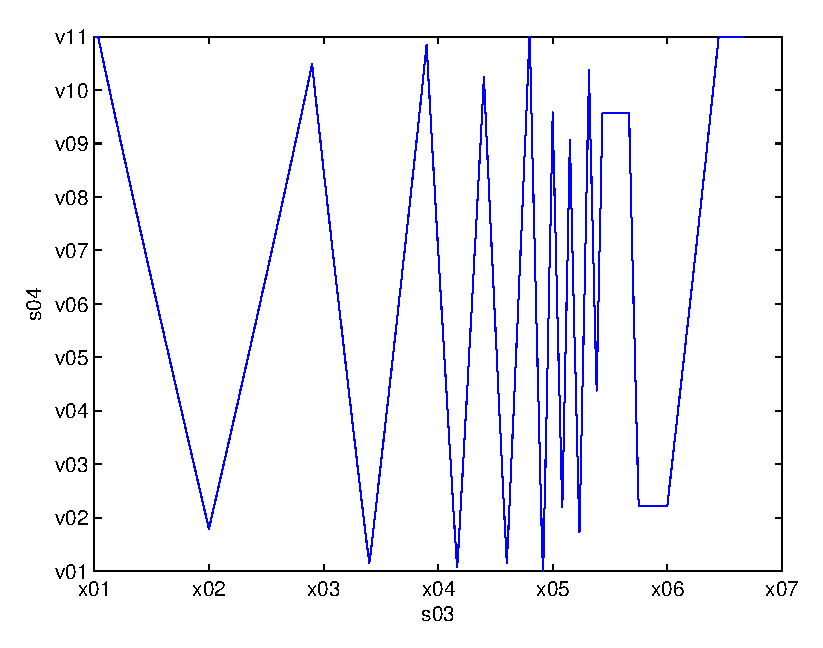
\includegraphics[width=15cm]{soc.eps}%
\end{psfrags}%
%
% End soc.tex
\end{document}
% See http://www.mathworks.de/matlabcentral/fileexchange/loadFile.do?objectId=4638
% for recent versions of laprint.m.
%
% created by:           LaPrint version 3.16 (13.9.2004)
% created on:           28-Mar-2014 11:35:41
% eps bounding box:     15 cm x 11.0893 cm
% comment:              
%
\begin{psfrags}%
\psfragscanon%
%
% text strings:
\psfrag{s03}[t][t]{\color[rgb]{0,0,0}\setlength{\tabcolsep}{0pt}\begin{tabular}{c}Time [hours]\end{tabular}}%
\psfrag{s04}[b][b]{\color[rgb]{0,0,0}\setlength{\tabcolsep}{0pt}\begin{tabular}{c}SOC\end{tabular}}%
%
% xticklabels:
\psfrag{x01}[t][t]{0}%
\psfrag{x02}[t][t]{5}%
\psfrag{x03}[t][t]{10}%
\psfrag{x04}[t][t]{15}%
\psfrag{x05}[t][t]{20}%
\psfrag{x06}[t][t]{25}%
\psfrag{x07}[t][t]{30}%
%
% yticklabels:
\psfrag{v01}[r][r]{0}%
\psfrag{v02}[r][r]{0.1}%
\psfrag{v03}[r][r]{0.2}%
\psfrag{v04}[r][r]{0.3}%
\psfrag{v05}[r][r]{0.4}%
\psfrag{v06}[r][r]{0.5}%
\psfrag{v07}[r][r]{0.6}%
\psfrag{v08}[r][r]{0.7}%
\psfrag{v09}[r][r]{0.8}%
\psfrag{v10}[r][r]{0.9}%
\psfrag{v11}[r][r]{1}%
%
% Figure:
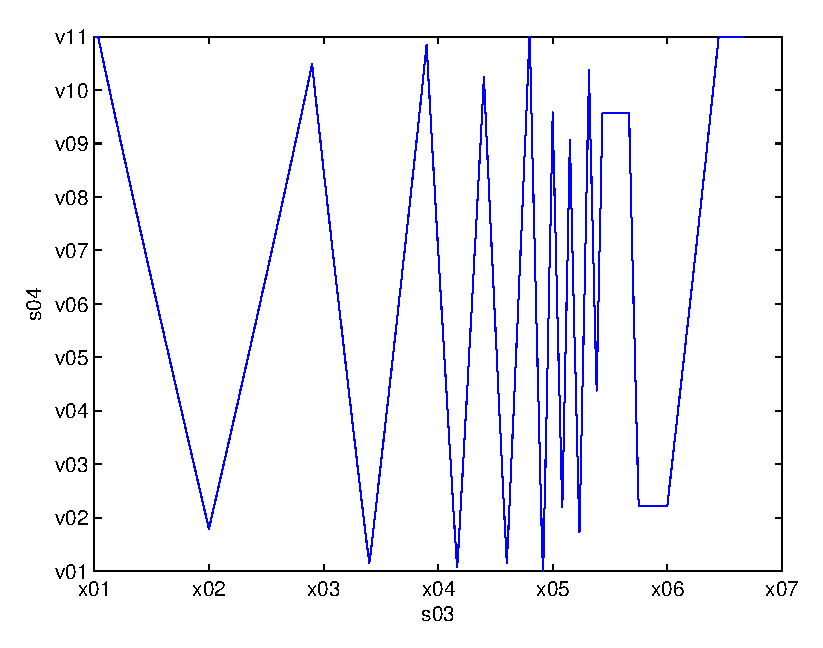
\includegraphics[width=15cm]{soc.eps}%
\end{psfrags}%
%
% End soc.tex
\end{document}
% See http://www.mathworks.de/matlabcentral/fileexchange/loadFile.do?objectId=4638
% for recent versions of laprint.m.
%
% created by:           LaPrint version 3.16 (13.9.2004)
% created on:           28-Mar-2014 11:35:41
% eps bounding box:     15 cm x 11.0893 cm
% comment:              
%
\begin{psfrags}%
\psfragscanon%
%
% text strings:
\psfrag{s03}[t][t]{\color[rgb]{0,0,0}\setlength{\tabcolsep}{0pt}\begin{tabular}{c}Time [hours]\end{tabular}}%
\psfrag{s04}[b][b]{\color[rgb]{0,0,0}\setlength{\tabcolsep}{0pt}\begin{tabular}{c}SOC\end{tabular}}%
%
% xticklabels:
\psfrag{x01}[t][t]{0}%
\psfrag{x02}[t][t]{5}%
\psfrag{x03}[t][t]{10}%
\psfrag{x04}[t][t]{15}%
\psfrag{x05}[t][t]{20}%
\psfrag{x06}[t][t]{25}%
\psfrag{x07}[t][t]{30}%
%
% yticklabels:
\psfrag{v01}[r][r]{0}%
\psfrag{v02}[r][r]{0.1}%
\psfrag{v03}[r][r]{0.2}%
\psfrag{v04}[r][r]{0.3}%
\psfrag{v05}[r][r]{0.4}%
\psfrag{v06}[r][r]{0.5}%
\psfrag{v07}[r][r]{0.6}%
\psfrag{v08}[r][r]{0.7}%
\psfrag{v09}[r][r]{0.8}%
\psfrag{v10}[r][r]{0.9}%
\psfrag{v11}[r][r]{1}%
%
% Figure:
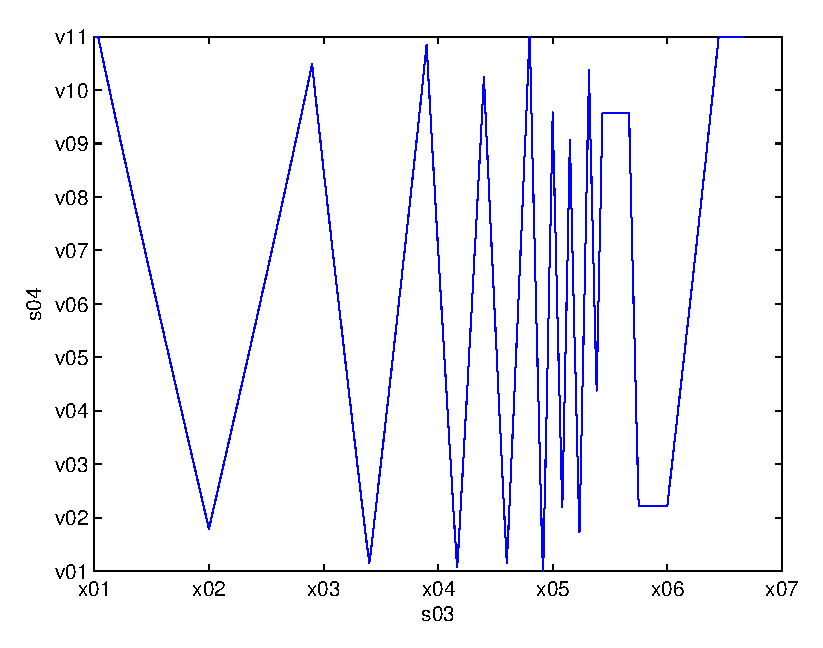
\includegraphics[width=15cm]{soc.eps}%
\end{psfrags}%
%
% End soc.tex

%\psfragfig[width=15cm]{chapter-2/figures/soc}
\pstool[width=15cm]{chapter-2/figures/soc}{% This file is generated by the MATLAB m-file laprint.m. It can be included
% into LaTeX documents using the packages graphicx, color and psfrag.
% It is accompanied by a postscript file. A sample LaTeX file is:
%    \documentclass{article}\usepackage{graphicx,color,psfrag}
%    \begin{document}% This file is generated by the MATLAB m-file laprint.m. It can be included
% into LaTeX documents using the packages graphicx, color and psfrag.
% It is accompanied by a postscript file. A sample LaTeX file is:
%    \documentclass{article}\usepackage{graphicx,color,psfrag}
%    \begin{document}% This file is generated by the MATLAB m-file laprint.m. It can be included
% into LaTeX documents using the packages graphicx, color and psfrag.
% It is accompanied by a postscript file. A sample LaTeX file is:
%    \documentclass{article}\usepackage{graphicx,color,psfrag}
%    \begin{document}\input{soc}\end{document}
% See http://www.mathworks.de/matlabcentral/fileexchange/loadFile.do?objectId=4638
% for recent versions of laprint.m.
%
% created by:           LaPrint version 3.16 (13.9.2004)
% created on:           28-Mar-2014 11:35:41
% eps bounding box:     15 cm x 11.0893 cm
% comment:              
%
\begin{psfrags}%
\psfragscanon%
%
% text strings:
\psfrag{s03}[t][t]{\color[rgb]{0,0,0}\setlength{\tabcolsep}{0pt}\begin{tabular}{c}Time [hours]\end{tabular}}%
\psfrag{s04}[b][b]{\color[rgb]{0,0,0}\setlength{\tabcolsep}{0pt}\begin{tabular}{c}SOC\end{tabular}}%
%
% xticklabels:
\psfrag{x01}[t][t]{0}%
\psfrag{x02}[t][t]{5}%
\psfrag{x03}[t][t]{10}%
\psfrag{x04}[t][t]{15}%
\psfrag{x05}[t][t]{20}%
\psfrag{x06}[t][t]{25}%
\psfrag{x07}[t][t]{30}%
%
% yticklabels:
\psfrag{v01}[r][r]{0}%
\psfrag{v02}[r][r]{0.1}%
\psfrag{v03}[r][r]{0.2}%
\psfrag{v04}[r][r]{0.3}%
\psfrag{v05}[r][r]{0.4}%
\psfrag{v06}[r][r]{0.5}%
\psfrag{v07}[r][r]{0.6}%
\psfrag{v08}[r][r]{0.7}%
\psfrag{v09}[r][r]{0.8}%
\psfrag{v10}[r][r]{0.9}%
\psfrag{v11}[r][r]{1}%
%
% Figure:
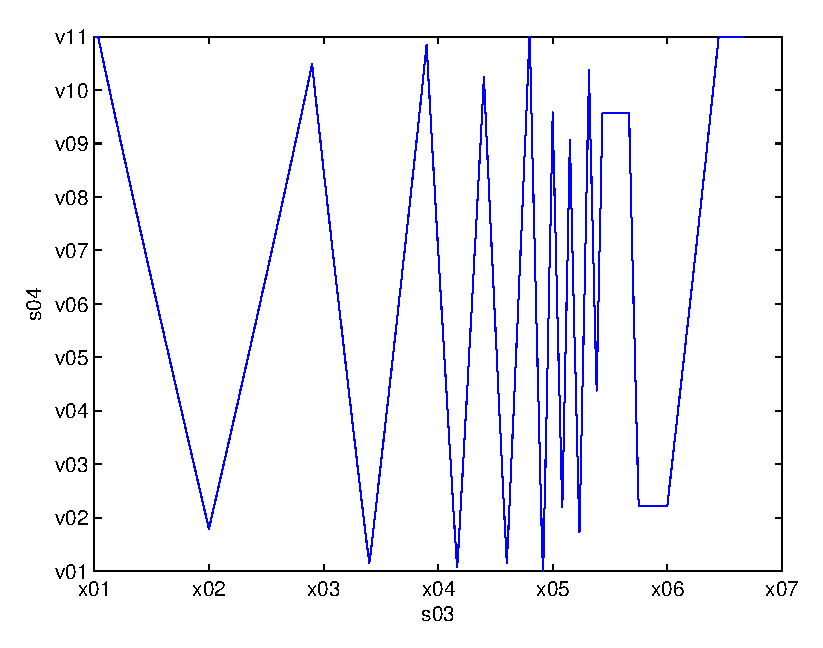
\includegraphics[width=15cm]{soc.eps}%
\end{psfrags}%
%
% End soc.tex
\end{document}
% See http://www.mathworks.de/matlabcentral/fileexchange/loadFile.do?objectId=4638
% for recent versions of laprint.m.
%
% created by:           LaPrint version 3.16 (13.9.2004)
% created on:           28-Mar-2014 11:35:41
% eps bounding box:     15 cm x 11.0893 cm
% comment:              
%
\begin{psfrags}%
\psfragscanon%
%
% text strings:
\psfrag{s03}[t][t]{\color[rgb]{0,0,0}\setlength{\tabcolsep}{0pt}\begin{tabular}{c}Time [hours]\end{tabular}}%
\psfrag{s04}[b][b]{\color[rgb]{0,0,0}\setlength{\tabcolsep}{0pt}\begin{tabular}{c}SOC\end{tabular}}%
%
% xticklabels:
\psfrag{x01}[t][t]{0}%
\psfrag{x02}[t][t]{5}%
\psfrag{x03}[t][t]{10}%
\psfrag{x04}[t][t]{15}%
\psfrag{x05}[t][t]{20}%
\psfrag{x06}[t][t]{25}%
\psfrag{x07}[t][t]{30}%
%
% yticklabels:
\psfrag{v01}[r][r]{0}%
\psfrag{v02}[r][r]{0.1}%
\psfrag{v03}[r][r]{0.2}%
\psfrag{v04}[r][r]{0.3}%
\psfrag{v05}[r][r]{0.4}%
\psfrag{v06}[r][r]{0.5}%
\psfrag{v07}[r][r]{0.6}%
\psfrag{v08}[r][r]{0.7}%
\psfrag{v09}[r][r]{0.8}%
\psfrag{v10}[r][r]{0.9}%
\psfrag{v11}[r][r]{1}%
%
% Figure:
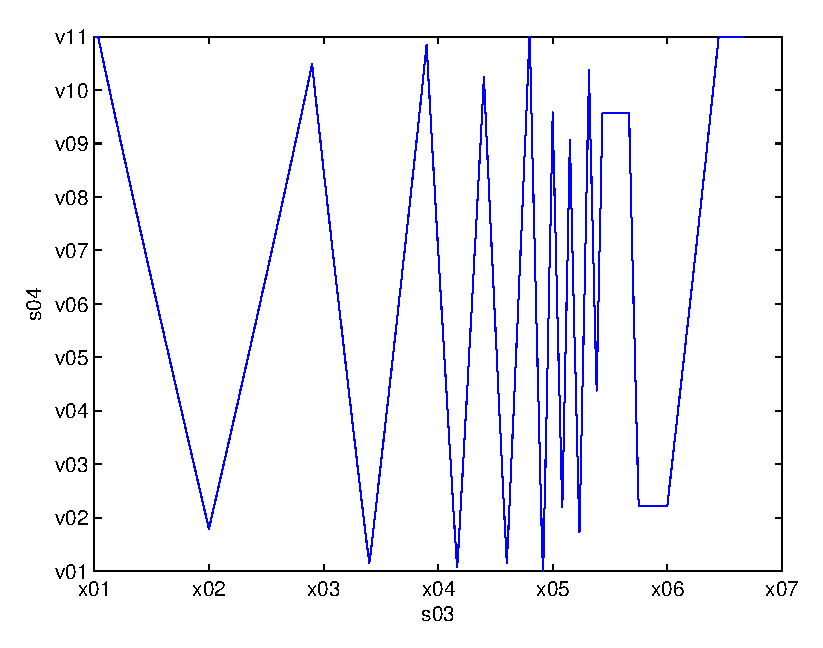
\includegraphics[width=15cm]{soc.eps}%
\end{psfrags}%
%
% End soc.tex
\end{document}
% See http://www.mathworks.de/matlabcentral/fileexchange/loadFile.do?objectId=4638
% for recent versions of laprint.m.
%
% created by:           LaPrint version 3.16 (13.9.2004)
% created on:           28-Mar-2014 11:35:41
% eps bounding box:     15 cm x 11.0893 cm
% comment:              
%
\begin{psfrags}%
\psfragscanon%
%
% text strings:
\psfrag{s03}[t][t]{\color[rgb]{0,0,0}\setlength{\tabcolsep}{0pt}\begin{tabular}{c}Time [hours]\end{tabular}}%
\psfrag{s04}[b][b]{\color[rgb]{0,0,0}\setlength{\tabcolsep}{0pt}\begin{tabular}{c}SOC\end{tabular}}%
%
% xticklabels:
\psfrag{x01}[t][t]{0}%
\psfrag{x02}[t][t]{5}%
\psfrag{x03}[t][t]{10}%
\psfrag{x04}[t][t]{15}%
\psfrag{x05}[t][t]{20}%
\psfrag{x06}[t][t]{25}%
\psfrag{x07}[t][t]{30}%
%
% yticklabels:
\psfrag{v01}[r][r]{0}%
\psfrag{v02}[r][r]{0.1}%
\psfrag{v03}[r][r]{0.2}%
\psfrag{v04}[r][r]{0.3}%
\psfrag{v05}[r][r]{0.4}%
\psfrag{v06}[r][r]{0.5}%
\psfrag{v07}[r][r]{0.6}%
\psfrag{v08}[r][r]{0.7}%
\psfrag{v09}[r][r]{0.8}%
\psfrag{v10}[r][r]{0.9}%
\psfrag{v11}[r][r]{1}%
%
% Figure:
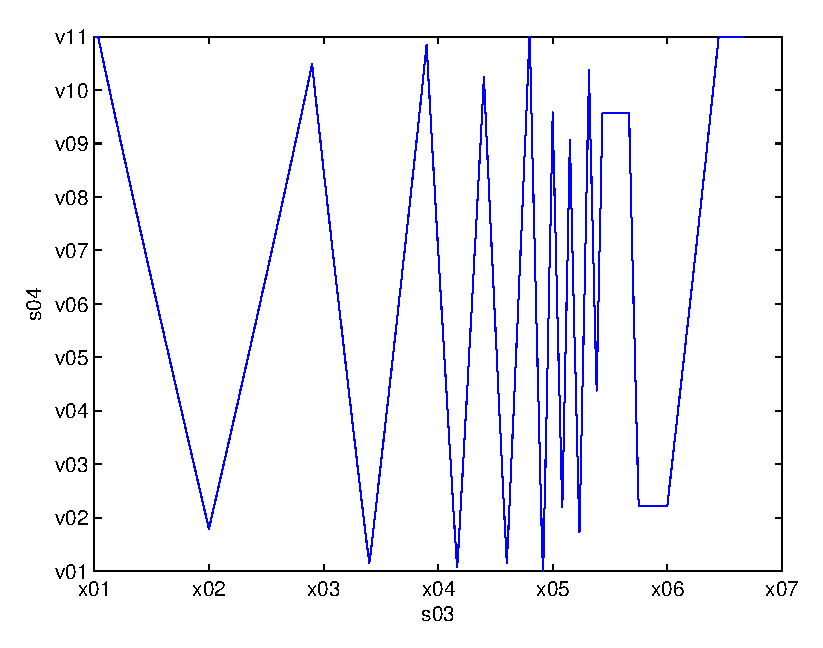
\includegraphics[width=15cm]{soc.eps}%
\end{psfrags}%
%
% End soc.tex
}
\caption{True SOC for one run due to input load.}
\label{fig:soc}
\end{figure}

\begin{figure}[htb]
\centering
%% This file is generated by the MATLAB m-file laprint.m. It can be included
% into LaTeX documents using the packages graphicx, color and psfrag.
% It is accompanied by a postscript file. A sample LaTeX file is:
%    \documentclass{article}\usepackage{graphicx,color,psfrag}
%    \begin{document}% This file is generated by the MATLAB m-file laprint.m. It can be included
% into LaTeX documents using the packages graphicx, color and psfrag.
% It is accompanied by a postscript file. A sample LaTeX file is:
%    \documentclass{article}\usepackage{graphicx,color,psfrag}
%    \begin{document}% This file is generated by the MATLAB m-file laprint.m. It can be included
% into LaTeX documents using the packages graphicx, color and psfrag.
% It is accompanied by a postscript file. A sample LaTeX file is:
%    \documentclass{article}\usepackage{graphicx,color,psfrag}
%    \begin{document}\input{meas}\end{document}
% See http://www.mathworks.de/matlabcentral/fileexchange/loadFile.do?objectId=4638
% for recent versions of laprint.m.
%
% created by:           LaPrint version 3.16 (13.9.2004)
% created on:           01-Apr-2014 19:01:39
% eps bounding box:     15 cm x 11.0893 cm
% comment:              
%
%\begin{psfrags}%
%\psfragscanon%
%
% text strings:
\psfrag{s03}[t][t]{\color[rgb]{0,0,0}\setlength{\tabcolsep}{0pt}\begin{tabular}{c}Time [hours]\end{tabular}}%
\psfrag{s04}[b][b]{\color[rgb]{0,0,0}\setlength{\tabcolsep}{0pt}\begin{tabular}{c}$V_\text{cell}$\ $[\text{V}]$\end{tabular}}%
%
% xticklabels:
\psfrag{x01}[t][t]{0}%
\psfrag{x02}[t][t]{5}%
\psfrag{x03}[t][t]{10}%
\psfrag{x04}[t][t]{15}%
\psfrag{x05}[t][t]{20}%
\psfrag{x06}[t][t]{25}%
\psfrag{x07}[t][t]{30}%
%
% yticklabels:
\psfrag{v01}[r][r]{1.5}%
\psfrag{v02}[r][r]{2}%
\psfrag{v03}[r][r]{2.5}%
\psfrag{v04}[r][r]{3}%
\psfrag{v05}[r][r]{3.5}%
\psfrag{v06}[r][r]{4}%
\psfrag{v07}[r][r]{4.5}%
\psfrag{v08}[r][r]{5}%
%
% Figure:
%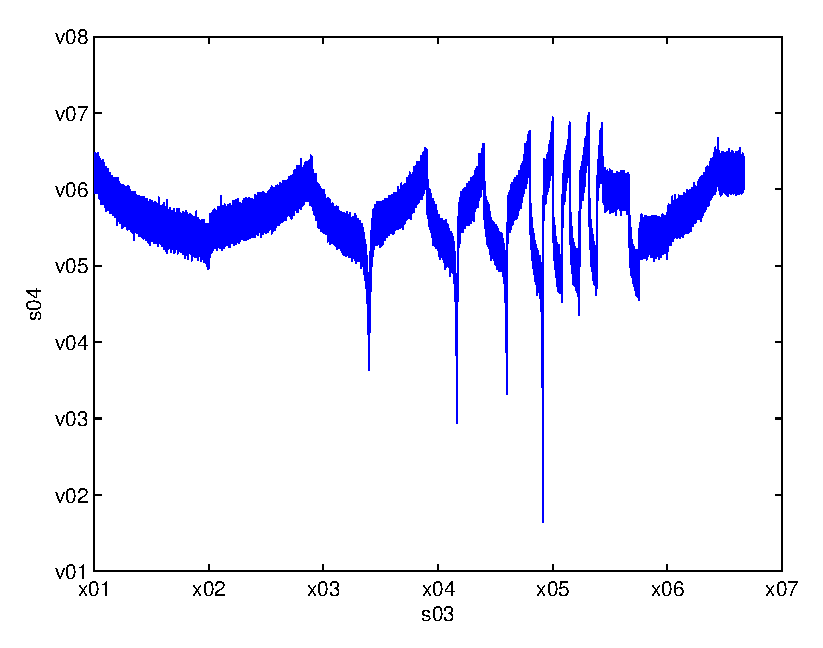
\includegraphics[width=15cm]{meas.eps}%
%\end{psfrags}%
%
% End meas.tex
\end{document}
% See http://www.mathworks.de/matlabcentral/fileexchange/loadFile.do?objectId=4638
% for recent versions of laprint.m.
%
% created by:           LaPrint version 3.16 (13.9.2004)
% created on:           01-Apr-2014 19:01:39
% eps bounding box:     15 cm x 11.0893 cm
% comment:              
%
%\begin{psfrags}%
%\psfragscanon%
%
% text strings:
\psfrag{s03}[t][t]{\color[rgb]{0,0,0}\setlength{\tabcolsep}{0pt}\begin{tabular}{c}Time [hours]\end{tabular}}%
\psfrag{s04}[b][b]{\color[rgb]{0,0,0}\setlength{\tabcolsep}{0pt}\begin{tabular}{c}$V_\text{cell}$\ $[\text{V}]$\end{tabular}}%
%
% xticklabels:
\psfrag{x01}[t][t]{0}%
\psfrag{x02}[t][t]{5}%
\psfrag{x03}[t][t]{10}%
\psfrag{x04}[t][t]{15}%
\psfrag{x05}[t][t]{20}%
\psfrag{x06}[t][t]{25}%
\psfrag{x07}[t][t]{30}%
%
% yticklabels:
\psfrag{v01}[r][r]{1.5}%
\psfrag{v02}[r][r]{2}%
\psfrag{v03}[r][r]{2.5}%
\psfrag{v04}[r][r]{3}%
\psfrag{v05}[r][r]{3.5}%
\psfrag{v06}[r][r]{4}%
\psfrag{v07}[r][r]{4.5}%
\psfrag{v08}[r][r]{5}%
%
% Figure:
%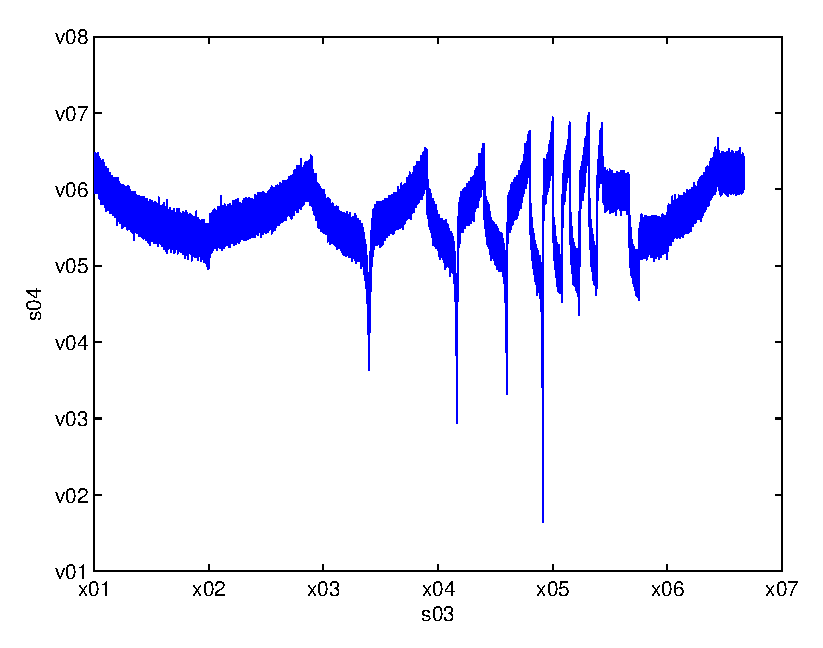
\includegraphics[width=15cm]{meas.eps}%
%\end{psfrags}%
%
% End meas.tex
\end{document}
% See http://www.mathworks.de/matlabcentral/fileexchange/loadFile.do?objectId=4638
% for recent versions of laprint.m.
%
% created by:           LaPrint version 3.16 (13.9.2004)
% created on:           01-Apr-2014 19:01:39
% eps bounding box:     15 cm x 11.0893 cm
% comment:              
%
%\begin{psfrags}%
%\psfragscanon%
%
% text strings:
\psfrag{s03}[t][t]{\color[rgb]{0,0,0}\setlength{\tabcolsep}{0pt}\begin{tabular}{c}Time [hours]\end{tabular}}%
\psfrag{s04}[b][b]{\color[rgb]{0,0,0}\setlength{\tabcolsep}{0pt}\begin{tabular}{c}$V_\text{cell}$\ $[\text{V}]$\end{tabular}}%
%
% xticklabels:
\psfrag{x01}[t][t]{0}%
\psfrag{x02}[t][t]{5}%
\psfrag{x03}[t][t]{10}%
\psfrag{x04}[t][t]{15}%
\psfrag{x05}[t][t]{20}%
\psfrag{x06}[t][t]{25}%
\psfrag{x07}[t][t]{30}%
%
% yticklabels:
\psfrag{v01}[r][r]{1.5}%
\psfrag{v02}[r][r]{2}%
\psfrag{v03}[r][r]{2.5}%
\psfrag{v04}[r][r]{3}%
\psfrag{v05}[r][r]{3.5}%
\psfrag{v06}[r][r]{4}%
\psfrag{v07}[r][r]{4.5}%
\psfrag{v08}[r][r]{5}%
%
% Figure:
%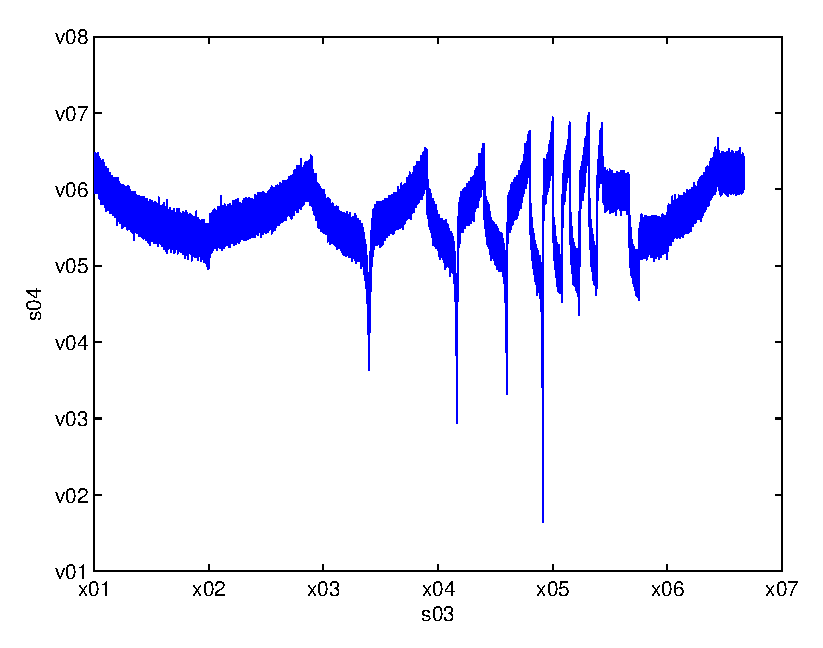
\includegraphics[width=15cm]{meas.eps}%
%\end{psfrags}%
%
% End meas.tex

%\psfragfig[width=15cm]{chapter-2/figures/meas}
\pstool[width=15cm]{chapter-2/figures/meas}{% This file is generated by the MATLAB m-file laprint.m. It can be included
% into LaTeX documents using the packages graphicx, color and psfrag.
% It is accompanied by a postscript file. A sample LaTeX file is:
%    \documentclass{article}\usepackage{graphicx,color,psfrag}
%    \begin{document}% This file is generated by the MATLAB m-file laprint.m. It can be included
% into LaTeX documents using the packages graphicx, color and psfrag.
% It is accompanied by a postscript file. A sample LaTeX file is:
%    \documentclass{article}\usepackage{graphicx,color,psfrag}
%    \begin{document}% This file is generated by the MATLAB m-file laprint.m. It can be included
% into LaTeX documents using the packages graphicx, color and psfrag.
% It is accompanied by a postscript file. A sample LaTeX file is:
%    \documentclass{article}\usepackage{graphicx,color,psfrag}
%    \begin{document}\input{meas}\end{document}
% See http://www.mathworks.de/matlabcentral/fileexchange/loadFile.do?objectId=4638
% for recent versions of laprint.m.
%
% created by:           LaPrint version 3.16 (13.9.2004)
% created on:           01-Apr-2014 19:01:39
% eps bounding box:     15 cm x 11.0893 cm
% comment:              
%
%\begin{psfrags}%
%\psfragscanon%
%
% text strings:
\psfrag{s03}[t][t]{\color[rgb]{0,0,0}\setlength{\tabcolsep}{0pt}\begin{tabular}{c}Time [hours]\end{tabular}}%
\psfrag{s04}[b][b]{\color[rgb]{0,0,0}\setlength{\tabcolsep}{0pt}\begin{tabular}{c}$V_\text{cell}$\ $[\text{V}]$\end{tabular}}%
%
% xticklabels:
\psfrag{x01}[t][t]{0}%
\psfrag{x02}[t][t]{5}%
\psfrag{x03}[t][t]{10}%
\psfrag{x04}[t][t]{15}%
\psfrag{x05}[t][t]{20}%
\psfrag{x06}[t][t]{25}%
\psfrag{x07}[t][t]{30}%
%
% yticklabels:
\psfrag{v01}[r][r]{1.5}%
\psfrag{v02}[r][r]{2}%
\psfrag{v03}[r][r]{2.5}%
\psfrag{v04}[r][r]{3}%
\psfrag{v05}[r][r]{3.5}%
\psfrag{v06}[r][r]{4}%
\psfrag{v07}[r][r]{4.5}%
\psfrag{v08}[r][r]{5}%
%
% Figure:
%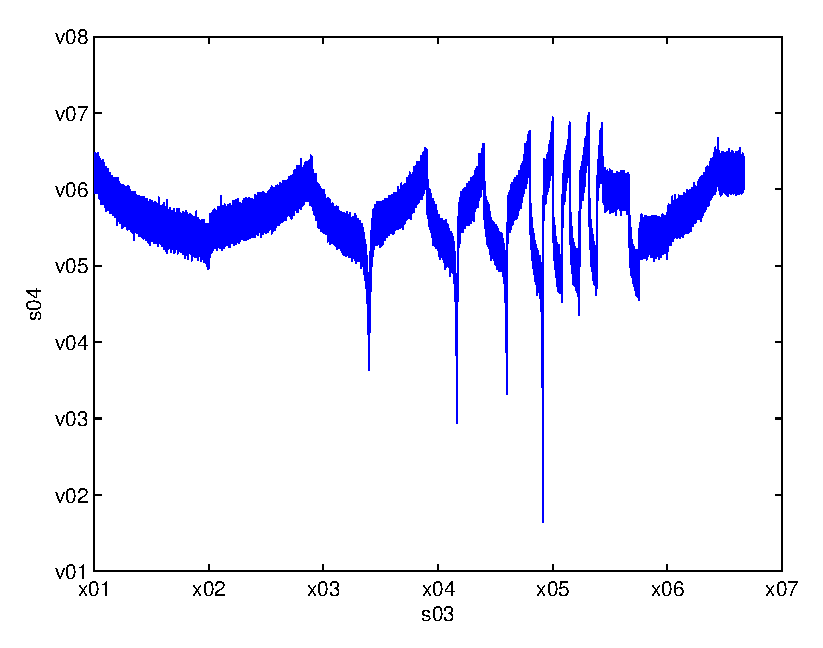
\includegraphics[width=15cm]{meas.eps}%
%\end{psfrags}%
%
% End meas.tex
\end{document}
% See http://www.mathworks.de/matlabcentral/fileexchange/loadFile.do?objectId=4638
% for recent versions of laprint.m.
%
% created by:           LaPrint version 3.16 (13.9.2004)
% created on:           01-Apr-2014 19:01:39
% eps bounding box:     15 cm x 11.0893 cm
% comment:              
%
%\begin{psfrags}%
%\psfragscanon%
%
% text strings:
\psfrag{s03}[t][t]{\color[rgb]{0,0,0}\setlength{\tabcolsep}{0pt}\begin{tabular}{c}Time [hours]\end{tabular}}%
\psfrag{s04}[b][b]{\color[rgb]{0,0,0}\setlength{\tabcolsep}{0pt}\begin{tabular}{c}$V_\text{cell}$\ $[\text{V}]$\end{tabular}}%
%
% xticklabels:
\psfrag{x01}[t][t]{0}%
\psfrag{x02}[t][t]{5}%
\psfrag{x03}[t][t]{10}%
\psfrag{x04}[t][t]{15}%
\psfrag{x05}[t][t]{20}%
\psfrag{x06}[t][t]{25}%
\psfrag{x07}[t][t]{30}%
%
% yticklabels:
\psfrag{v01}[r][r]{1.5}%
\psfrag{v02}[r][r]{2}%
\psfrag{v03}[r][r]{2.5}%
\psfrag{v04}[r][r]{3}%
\psfrag{v05}[r][r]{3.5}%
\psfrag{v06}[r][r]{4}%
\psfrag{v07}[r][r]{4.5}%
\psfrag{v08}[r][r]{5}%
%
% Figure:
%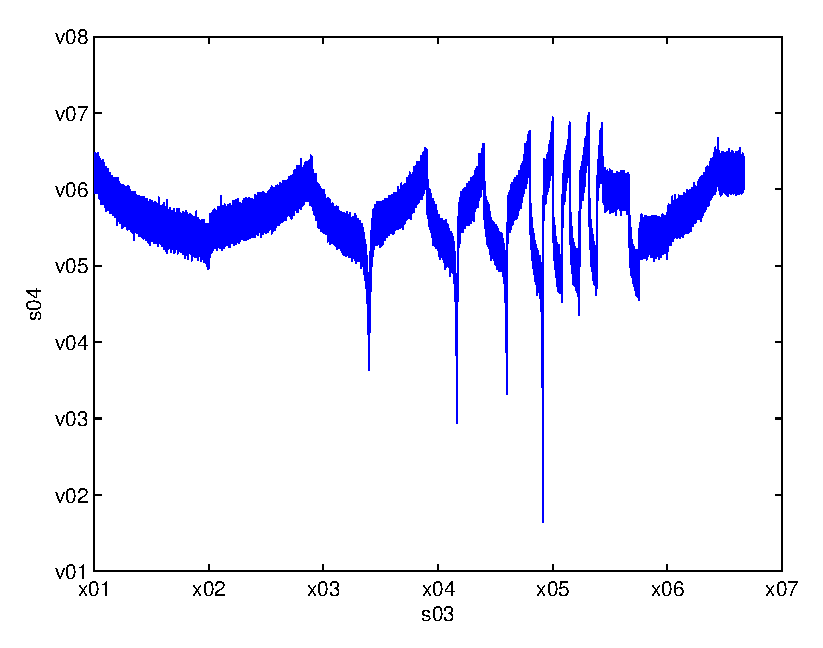
\includegraphics[width=15cm]{meas.eps}%
%\end{psfrags}%
%
% End meas.tex
\end{document}
% See http://www.mathworks.de/matlabcentral/fileexchange/loadFile.do?objectId=4638
% for recent versions of laprint.m.
%
% created by:           LaPrint version 3.16 (13.9.2004)
% created on:           01-Apr-2014 19:01:39
% eps bounding box:     15 cm x 11.0893 cm
% comment:              
%
%\begin{psfrags}%
%\psfragscanon%
%
% text strings:
\psfrag{s03}[t][t]{\color[rgb]{0,0,0}\setlength{\tabcolsep}{0pt}\begin{tabular}{c}Time [hours]\end{tabular}}%
\psfrag{s04}[b][b]{\color[rgb]{0,0,0}\setlength{\tabcolsep}{0pt}\begin{tabular}{c}$V_\text{cell}$\ $[\text{V}]$\end{tabular}}%
%
% xticklabels:
\psfrag{x01}[t][t]{0}%
\psfrag{x02}[t][t]{5}%
\psfrag{x03}[t][t]{10}%
\psfrag{x04}[t][t]{15}%
\psfrag{x05}[t][t]{20}%
\psfrag{x06}[t][t]{25}%
\psfrag{x07}[t][t]{30}%
%
% yticklabels:
\psfrag{v01}[r][r]{1.5}%
\psfrag{v02}[r][r]{2}%
\psfrag{v03}[r][r]{2.5}%
\psfrag{v04}[r][r]{3}%
\psfrag{v05}[r][r]{3.5}%
\psfrag{v06}[r][r]{4}%
\psfrag{v07}[r][r]{4.5}%
\psfrag{v08}[r][r]{5}%
%
% Figure:
%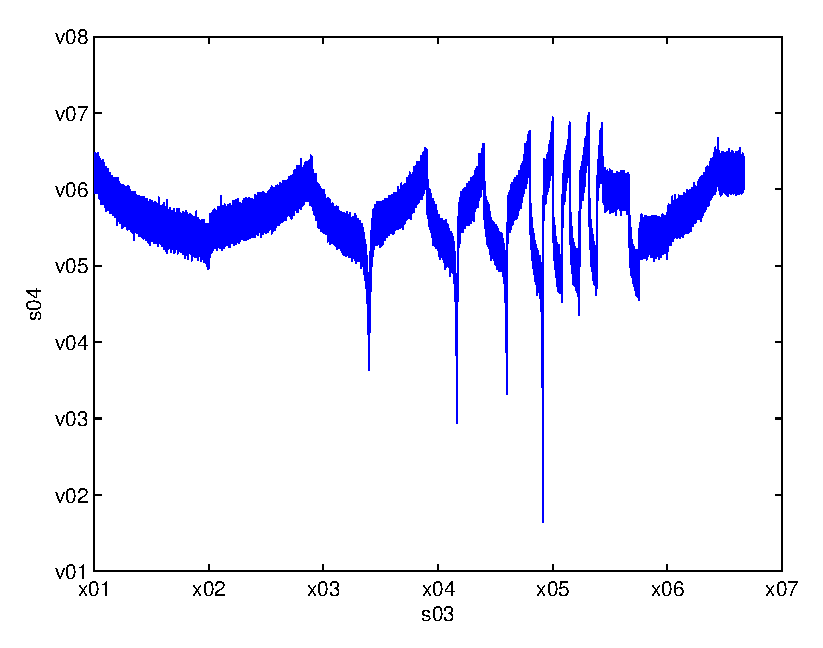
\includegraphics[width=15cm]{meas.eps}%
%\end{psfrags}%
%
% End meas.tex
}
\caption{Noisy measurement $V_\text{cell}$ for one run.}
\label{fig:meas}
\end{figure}

The Monte Carlo trials used varying sampling periods, calculated as some multiple $K$ of the simulation step size. For example, for a desired sampling period of 300 seconds, the actual sampling period is
\begin{equation}
    T_s = K \delta_\text{sim} = 1826 \times 0.164255~\text{s} = 299.93~\text{s},
\end{equation}
where the factor $K$ is chosen to minimize the difference between the desired and actual periods. For convenience, the sampling period will refer to the actual sampling period calculated in this manner. The sampling periods used in this study were $T_s=30$, 150, and 300 seconds.

\section{Filtering Setup}

This thesis studied five filters, namely the EKF, UKF, third-order CKF (CKF3), fifth-order CKF (CKF5), and SLF. The EKF used \crefrange{eq:ekfpredx}{eq:ekf_l}. The UKF used \crefrange{eq:ukfp1}{eq:ukful} along with the changes in \cref{eq:ukf_c1,eq:ukf_c2}. The CKF3 used \crefrange{eq:cr3_1}{eq:cr3_l} along with the change in \cref{eq:ckf3_c}. The CKF5 used \crefrange{eq:cr5_1}{eq:cr5_l} along with the change in \cref{eq:ckf5_c}. Finally, the SLF used \cref{eq:slf1,eq:slfl}.

The filters used in this study were implemented in Fortran for speed reasons. The programs used LAPACK 3.5.0 and were compiled using gfortran 4.8 for a 32-bit Cygwin environment on a computer running 64-bit Windows 7 with optimization flags of \texttt{-O3}. Due to the large size of the data, the input and output were performed using files. The time measurements were of the CPU time used by the filters, disregarding the time taken to read and write the data. The use of CPU time results in less
variability between runs. Additionally, to increase the accuracy of the discretized integration in the prediction steps, the sampling period is divided by a positive integer $M$ and the integration is performed in $M$ steps. Thus, the prediction and update portions of the filters can be calculated at different rates.

The formulas used to implement the filters were already described in Chapter 1. The only filter with tunable parameters was the UKF. Parameter values of $\alpha=0.05$, $\beta=2$, and $\kappa=0$ were used, where the values were chosen to be the typical values for a Gaussian distribution. It was noticed that $\alpha$ could not be too small for this problem; otherwise, the covariance matrix quickly loses positive definiteness. The choice of $\alpha$ was a compromise between the typical
choice of a small value and the stability gained from a larger value. Additionally, as $\alpha$ approaches 1, the UKF becomes very similar to the third-order CKF used by this thesis, so the chosen value is on the small side to better differentiate the two filters. The filtering was performed assuming an initial state of $x_0=[1,0,0]^\top$ and an initial covariance matrix of $P_0=10^{-6} I_3$, where the initial state was chosen to match the actual state and the initial covariance was experimentally tuned for fast convergence. 

\end{document}
